\documentclass[english]{beamer}
\usetheme{Madrid}
\usepackage{fancyhdr, amsfonts, amssymb, amsthm, amsmath, MnSymbol, wasysym, bbm, mathrsfs, graphicx, listings, parskip, float, hyperref, booktabs}
\def\Z{\mathbb{Z}}
\def\R{\mathbb{R}}
\def\Q{\mathbb{Q}}
\def\N{\mathbb{N}}
\def\C{\mathbb{C}}
\def\P{\mathbb{P}}
\def\E{\mathbb{E}}
\def\ind{\mathbbm{1}}
\def\giv{{\,|\,}}
\def\lf{\left\lfloor}
\def\rf{\right\rfloor}
\def\lc{\left\lceil}
\def\rc{\right\rceil}
\def\var{\text{Var}}
\newcommand{\simiid}{\overset{\textrm{i.i.d.}}{\sim}}
\newcommand{\simind}{\overset{\textrm{ind.}}{\sim}}
\newcommand{\indep}{\raisebox{0.05em}{\rotatebox[origin=c]{90}{$\models$}}}

% 3x3 matrix code
% $$ \left( \begin{array}{ccc}
% a & b & c \\
% d & e & f \\
% g & h & i \end{array} \right)$$

% formula in array
% $$ |x| = \left\{ \begin{array}{ll}
%        x & \mbox{if $x \geq 0$};\\
%        -x & \mbox{if $x < 0$}. \end{array} \right. $$

\title[]{The Effect of Vaccination on Hospital Admission}
\subtitle{\small \url{https://github.com/erickim/PH252D\_final\_project}}
\author[Dukhovnov, Duncan, Kim, Proudman]{Denys Dukhovnov, James Duncan, Eric Kim, David Proudman}
\date{April 30, 2018}

\begin{document}
\begin{frame}
\titlepage
\end{frame}

\begin{frame}{Introduction}
\begin{itemize}
\item Americans $\geq$65 have some of the highest immunization rates among other age groups in the country
\item Seasonal Influenza vaccine is the most common type with 63.4$\%$ of adults over 65 getting the vaccine (2015-2016)\footnote{\tiny{Centers for Disease Control and Prevention. Recommended Vaccines for Adults. https://www.cdc.gov/vaccines/ adults/rec-vac/index.html. Published January 25, 2018. Accessed April 17, 2018}} 
\item The elderly subpopulation with type 2 diabetes must take additional precautions to due to comorbidities, such as various heart and respiratory tract conditions, among other
\end{itemize}
\end{frame}

\begin{frame}{Introduction (cont.)}
\begin{itemize}
\item By 2015 the overall hospitalization rates among $\geq$65 have decreased to 26,400 from 35,214 per 100,000 in 2000 (25$\%$ decrease)\footnote{\tiny{Sun R, Karaca Z, Wong HS. Trends in Hospital Inpatient Stays by Age and Payer, 2000-2015. Rockville, MD: Agency for Healthcare Research and Quality; 2018. https://www.hcup-us.ahrq.gov/reports/statbriefs/sb235-Inpatient-Stays-Age- Payer-Trends.jsp. Accessed April 23, 2018.}}
\item Hospitalization rates for cardiac and stroke, cerebrovascular disease, pneumonia/influenza, and other cause-of-death related conditions in the unvaccinated population $\geq$65 are close to 3$\%$ during the influenza season, but get significantly reduced to 2.2$\%$ for the seasonal influenza vaccine recipients\footnote{\tiny{Nichol KL et al. Influenza Vaccination and Reduction in Hospitalizations for Cardiac Disease and Stroke among the Elderly. \textit{N Engl J Med}. 2003;348(14):1322-1332.}}
\end{itemize}
\end{frame}

\begin{frame}{Scientific Question}
What is the effect of [any] vaccination in 2015 on hospital admission [for any reason] in 2016 among the older adults over 65 years old, diagnosed with diabetes?
\end{frame}

\begin{frame}{The Causal Model and Target Causal Parameter}
\centerline{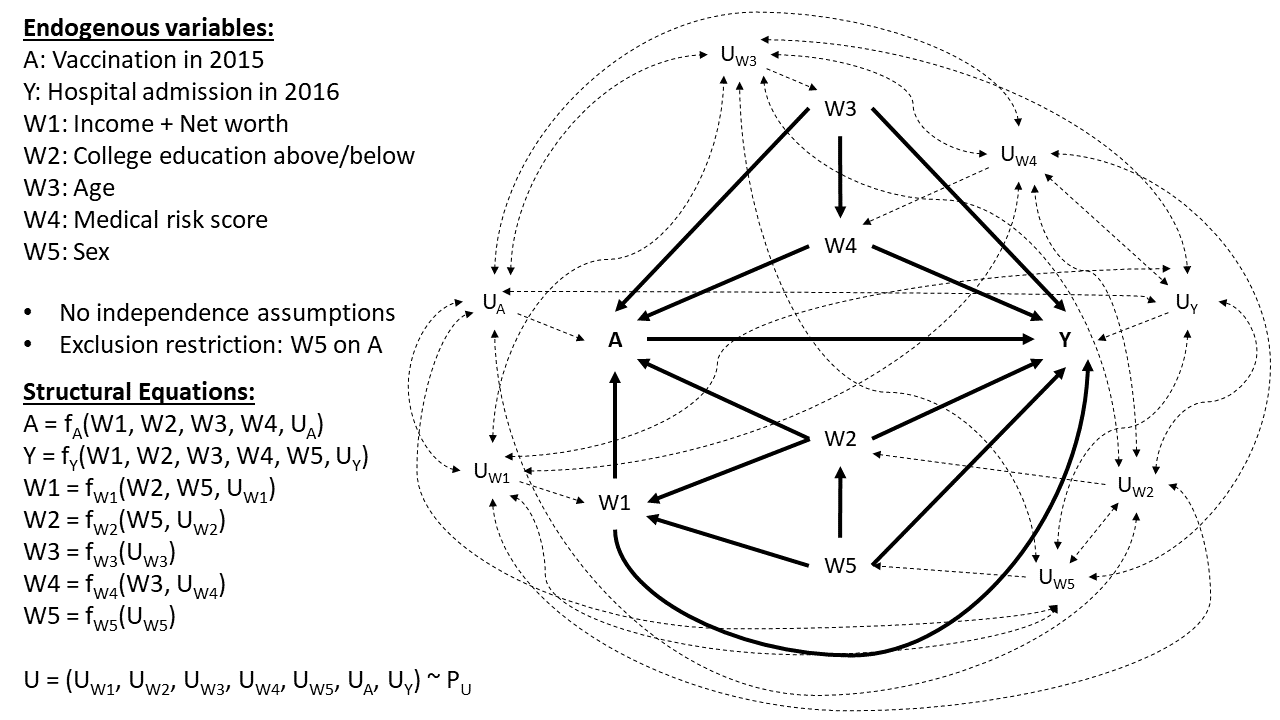
\includegraphics[scale=.275]{figures/DAG.PNG}}
\footnotesize Our target causal parameter is the average treatment effect
$$\Psi^F(P_{U,X}) = \E_{U,X}[Y_1-Y_0]$$
\footnotesize Where the counterfactual variables of interest is the number of hospital admissions under vaccination and in the absence of vaccinations.
\end{frame}

\begin{frame}{Observed Data}
\begin{table}
\resizebox{\columnwidth}{!}{%
\begin{tabular}{llccccccc}
\toprule
& & \multicolumn{2}{c}{Vaccinated} & \multicolumn{2}{c}{Gender} & \multicolumn{2}{c}{College} & \multicolumn{1}{c}{} \\ \cmidrule(lr){3-4}\cmidrule(lr){5-6}\cmidrule(lr){7-8}
 &  & N & Y & F & M & N & Y & \multicolumn{1}{c}{Overall} \\ 
\midrule
 & count  & $20904$ & $\phantom{0}5875$ & $14055$ & $12724$ & $24843$ & $\phantom{0}1936$ & $26779$ \\
 & \% in stratum  & $78.06\%$ & $21.94\%$ & $52.48\%$ & $47.51\%$ & $92.77\%$ & $\phantom{0}7.23\%$ & $100\%$ \\
Wealth Index & mean  & $11.73$ & $11.94$ & $11.54$ & $12.03$ & $11.75$ & $12.10$ & $\phantom{0}11.78$ \\
 & sd  & $\phantom{0}1.51$ & $\phantom{0}1.53$ & $\phantom{0}1.57$ & $\phantom{0}1.41$ & $\phantom{0}1.51$ & $\phantom{0}1.48$ & $\phantom{00}1.51$ \\
Age & mean  & $74.66$ & $74.68$ & $74.87$ & $74.43$ & $74.75$ & $73.51$ & $\phantom{0}74.66$ \\
 & sd  & $\phantom{0}6.61$ & $\phantom{0}6.32$ & $\phantom{0}6.74$ & $\phantom{0}6.32$ & $\phantom{0}6.57$ & $\phantom{0}6.11$ & $\phantom{00}6.55$ \\
 Medical Risk Score & mean  & $\phantom{0}1.20$ & $\phantom{0}1.11$ & $\phantom{0}1.17$ & $\phantom{0}1.19$ & $\phantom{0}1.18$ & $\phantom{0}1.10$ & $\phantom{00}1.18$ \\
 & sd  & $\phantom{0}0.98$ & $\phantom{0}0.87$ & $\phantom{0}0.94$ & $\phantom{0}0.98$ & $\phantom{0}0.96$ & $\phantom{0}0.96$ & $\phantom{00}0.96$ \\
No. Hospital Visits & mean  & $\phantom{0}0.34$ & $\phantom{0}0.29$ & $\phantom{0}0.32$ & $\phantom{0}0.33$ & $\phantom{0}0.33$ & $\phantom{0}0.28$ & $\phantom{00}0.33$ \\
 & sd  & $\phantom{0}0.94$ & $\phantom{0}0.83$ & $\phantom{0}0.90$ & $\phantom{0}0.93$ & $\phantom{0}0.92$ & $\phantom{0}0.86$ & $\phantom{00}0.92$ \\
\bottomrule 
\end{tabular}
}
\end{table}
\end{frame}
\begin{frame}{Observed Data (cont.)}
\begin{table}
\resizebox{\columnwidth}{!}{%
\begin{tabular}{llcccccccc}
\toprule
& & \multicolumn{8}{c}{Vaccinated} \\ \cmidrule(lr){3-10}
& & \multicolumn{4}{c}{No} & \multicolumn{4}{c}{Yes} \\ \cmidrule(lr){3-6}\cmidrule(lr){7-10}
& & \multicolumn{4}{c}{Gender} & \multicolumn{4}{c}{Gender} \\ \cmidrule(lr){3-6}\cmidrule(lr){7-10}
& & \multicolumn{2}{c}{F} & \multicolumn{2}{c}{M} & \multicolumn{2}{c}{F} & \multicolumn{2}{c}{M} \\ \cmidrule(lr){3-4}\cmidrule(lr){5-6}\cmidrule(lr){7-8}\cmidrule(lr){9-10}
& & \multicolumn{2}{c}{College} & \multicolumn{2}{c}{College} & \multicolumn{2}{c}{College} & \multicolumn{2}{c}{College} \\ \cmidrule(lr){3-4}\cmidrule(lr){5-6}\cmidrule(lr){7-8}\cmidrule(lr){9-10}
 &  & N & Y & N & Y & N & Y & N & \multicolumn{1}{c}{Y} \\ 
\midrule
& count & 10133 & 763 & 9308 & 700 & 2901 & 258 & 2501 & 215 \\
 & \% of total & $37.84\%$ & $2.85\%$ & $34.76\%$ & $2.61\%$ & $10.83\%$ & $0.96\%$ & $9.34\%$ & $0.80\%$ \\
Wealth Index & mean  & $11.47$ & $11.79$ & $11.97$ & $12.27$ & $11.70$ & $12.18$ & $12.15$ & $12.55$ \\
 & sd & $\phantom{0}1.56$ & $\phantom{0}1.52$ & $\phantom{0}1.39$ & $\phantom{0}1.44$ & $\phantom{0}1.58$ & $\phantom{0}1.43$ & $\phantom{0}1.44$ & $\phantom{0}1.34$ \\
Age & mean  & $75.01$ & $73.18$ & $74.45$ & $73.82$ & $74.95$ & $73.42$ & $74.58$ & $73.80$ \\
 & sd  & $\phantom{0}6.83$ & $\phantom{0}6.05$ & $\phantom{0}6.40$ & $\phantom{0}6.28$ & $\phantom{0}6.60$ & $\phantom{0}5.91$ & $\phantom{0}6.04$ & $\phantom{0}6.01$ \\
 Medical Risk Score & mean  & $\phantom{0}1.20$ & $\phantom{0}1.12$ & $\phantom{0}1.20$ & $\phantom{0}1.10$ & $\phantom{0}1.09$ & $\phantom{0}1.00$ & $\phantom{0}1.15$ & $\phantom{0}1.16$ \\
 & sd  & $\phantom{0}0.96$ & $\phantom{0}0.97$ & $\phantom{0}1.00$ & $\phantom{0}1.01$ & $\phantom{0}0.86$ & $\phantom{0}0.81$ & $\phantom{0}0.90$ & $\phantom{0}0.92$ \\
No. Hospital Visits & mean  & $\phantom{0}0.34$ & $\phantom{0}0.30$ & $\phantom{0}0.34$ & $\phantom{0}0.30$ & $\phantom{0}0.28$ & $\phantom{0}0.17$ & $\phantom{0}0.31$ & $\phantom{0}0.25$ \\
 & sd  & $\phantom{0}0.93$ & $\phantom{0}0.95$ & $\phantom{0}0.95$ & $\phantom{0}0.92$ & $\phantom{0}0.82$ & $\phantom{0}0.50$ & $\phantom{0}0.88$ & $\phantom{0}0.66$ \\
\bottomrule 
\end{tabular}
}
\end{table}
\end{frame}

\begin{frame}{Identifiability}
Under the current model the target causal parameter is not identifiable. But given background knowledge, some independence assumptions can be established.\\
$U_{A} \indep U_{W_{3}}, U_{W_{5}}$ \\
$U_{Y} \indep U_{W_{1}}, U_{W_{2}}, U_{W_{3}}, U_{W_{5}}$ \\
$U_{W_{1}} \indep U_{W_{3}}, U_{W_{4}}, U_{W_{5}}, U_{Y}$ \\
$U_{W_{2}} \indep U_{W_{3}}, U_{W_{4}}, U_{W_{5}}, U_{Y}$ \\
$U_{W_{3}} \indep U_{A}, U_{W_{1}}, U_{W_{2}}, U_{W_{4}}, U_{W_{5}}, U_{Y}$ \\
$U_{W_{4}} \indep U_{W_{1}}, U_{W_{2}}, U_{W_{3}}, U_{W_{5}}$ \\
$U_{W_{5}} \indep U_{A}, U_{W_{1}}, U_{W_{2}}, U_{W_{3}}, U_{W_{4}}, U_{Y}$
\par
Knowledge is insufficient. Further convenience assumptions are required for identifiability, under the backdoor criterion and randomization assumptions.  
\par
$U_{A} \indep U_{Y}, U_{W_{3}}, U_{W_{4}}, U_{W_{5}}$ \\
$U_{Y} \indep U_{A}, U_{W_{3}}, U_{W_{5}}$
\end{frame}

\begin{frame}{Identifiability (cont.)}
\centerline{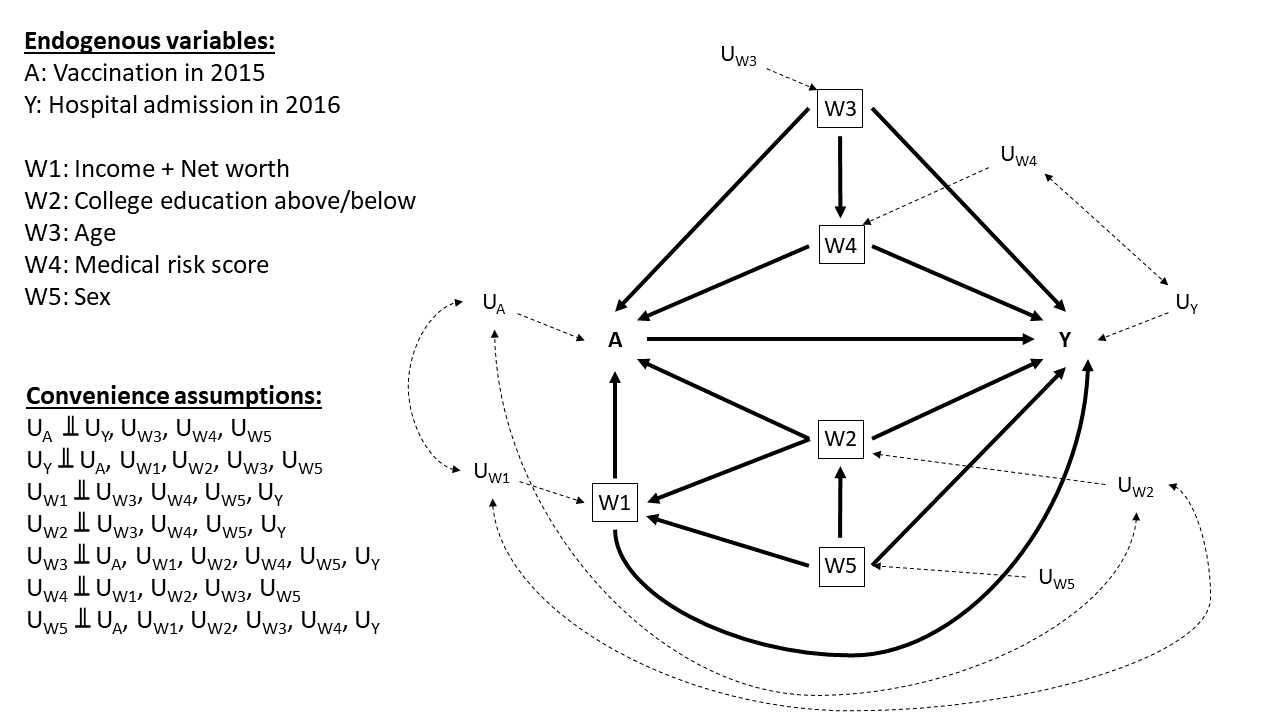
\includegraphics[scale=.38]{figures/DAG_identifiable.png}}
\end{frame}

\begin{frame}{Statistical Model and Estimand}
Our statistical model is a semi-parametric model where we take the previous assumptions on identifiability as restrictions on our observed data distributions $P_0$. 

Our estimands for the Average Treatment Effect will be the G-Computation, IPTW, Stabilized IPTW, and TMLE estimators.
\end{frame}

\begin{frame}{Math Review}
\begin{block}{G-computation Estimator}
The G-computation/simple substitution estimator is as follows
$$\hat{\Psi}(\P_n) = \frac{1}{n} \sum_{i=1}^n \bigg[ \hat{\E}\Big(Y_i \giv A_i = 1, \overrightarrow{W}_i\Big) - \hat{\E}\Big(Y_i \giv A_i = 0, \overrightarrow{W}_i\Big) \bigg]$$
\end{block}

\begin{block}{IPTW Estimator}
The IPTW substitution estimator is as follows (similar to Horvitz-Thompson estimator)
$$\hat{\Psi}(\P_n) = \frac{1}{n} \sum_{i=1}^n \frac{\ind\{A_i = 1\}}{g(A_i \giv W_i)} Y_i - \frac{1}{n} \sum_{i=1}^n \frac{\ind\{A_i = 0 \}}{g(A_i \giv W_i)} Y_i$$
\end{block}
\end{frame}

\begin{frame}{More Math Review}
\begin{block}{Stabilized IPTW Estimator}
The Stabilized IPTW substitution estimator is as follows (similar to Hajek estimator
$$\hat{\Psi}(\P_n) = \frac{\sum_{i=1}^n \frac{\ind\{A_i = 1\}}{g(A_i \giv W_i)} Y_i}{\sum_{j=1}^n \frac{\ind\{A_j = 1\}}{g(A_j \giv W_j)}} - \frac{\sum_{i=1}^n \frac{\ind\{A_i = 0 \}}{g(A_i \giv W_i)}Y_i}{\sum_{j=1}^n \frac{\ind\{A_j = 0\}}{g(A_j \giv W_j)}}$$
\end{block}

\begin{block}{Targeted Maximum Likelihood Estimator}
The TMLE estimator is defined to be the solution to the efficient influence curve
$$0 = \frac{1}{n} \sum_{i=1}^n D^*(P_n^*)(O_i)$$
Where $D^*$ is the efficient influence curve as follows
$$D^*(P) = \left[\frac{A}{g(A \giv W)} - \frac{1-A}{g(0 \giv W)}\right][Y-\overline{Q}(A,W)] + \overline{Q}(1, W) - \overline{Q}(0,W) - \psi$$
\end{block}
\end{frame}

\begin{frame}{Positivity Assumption}
\begin{minipage}{0.5\columnwidth}
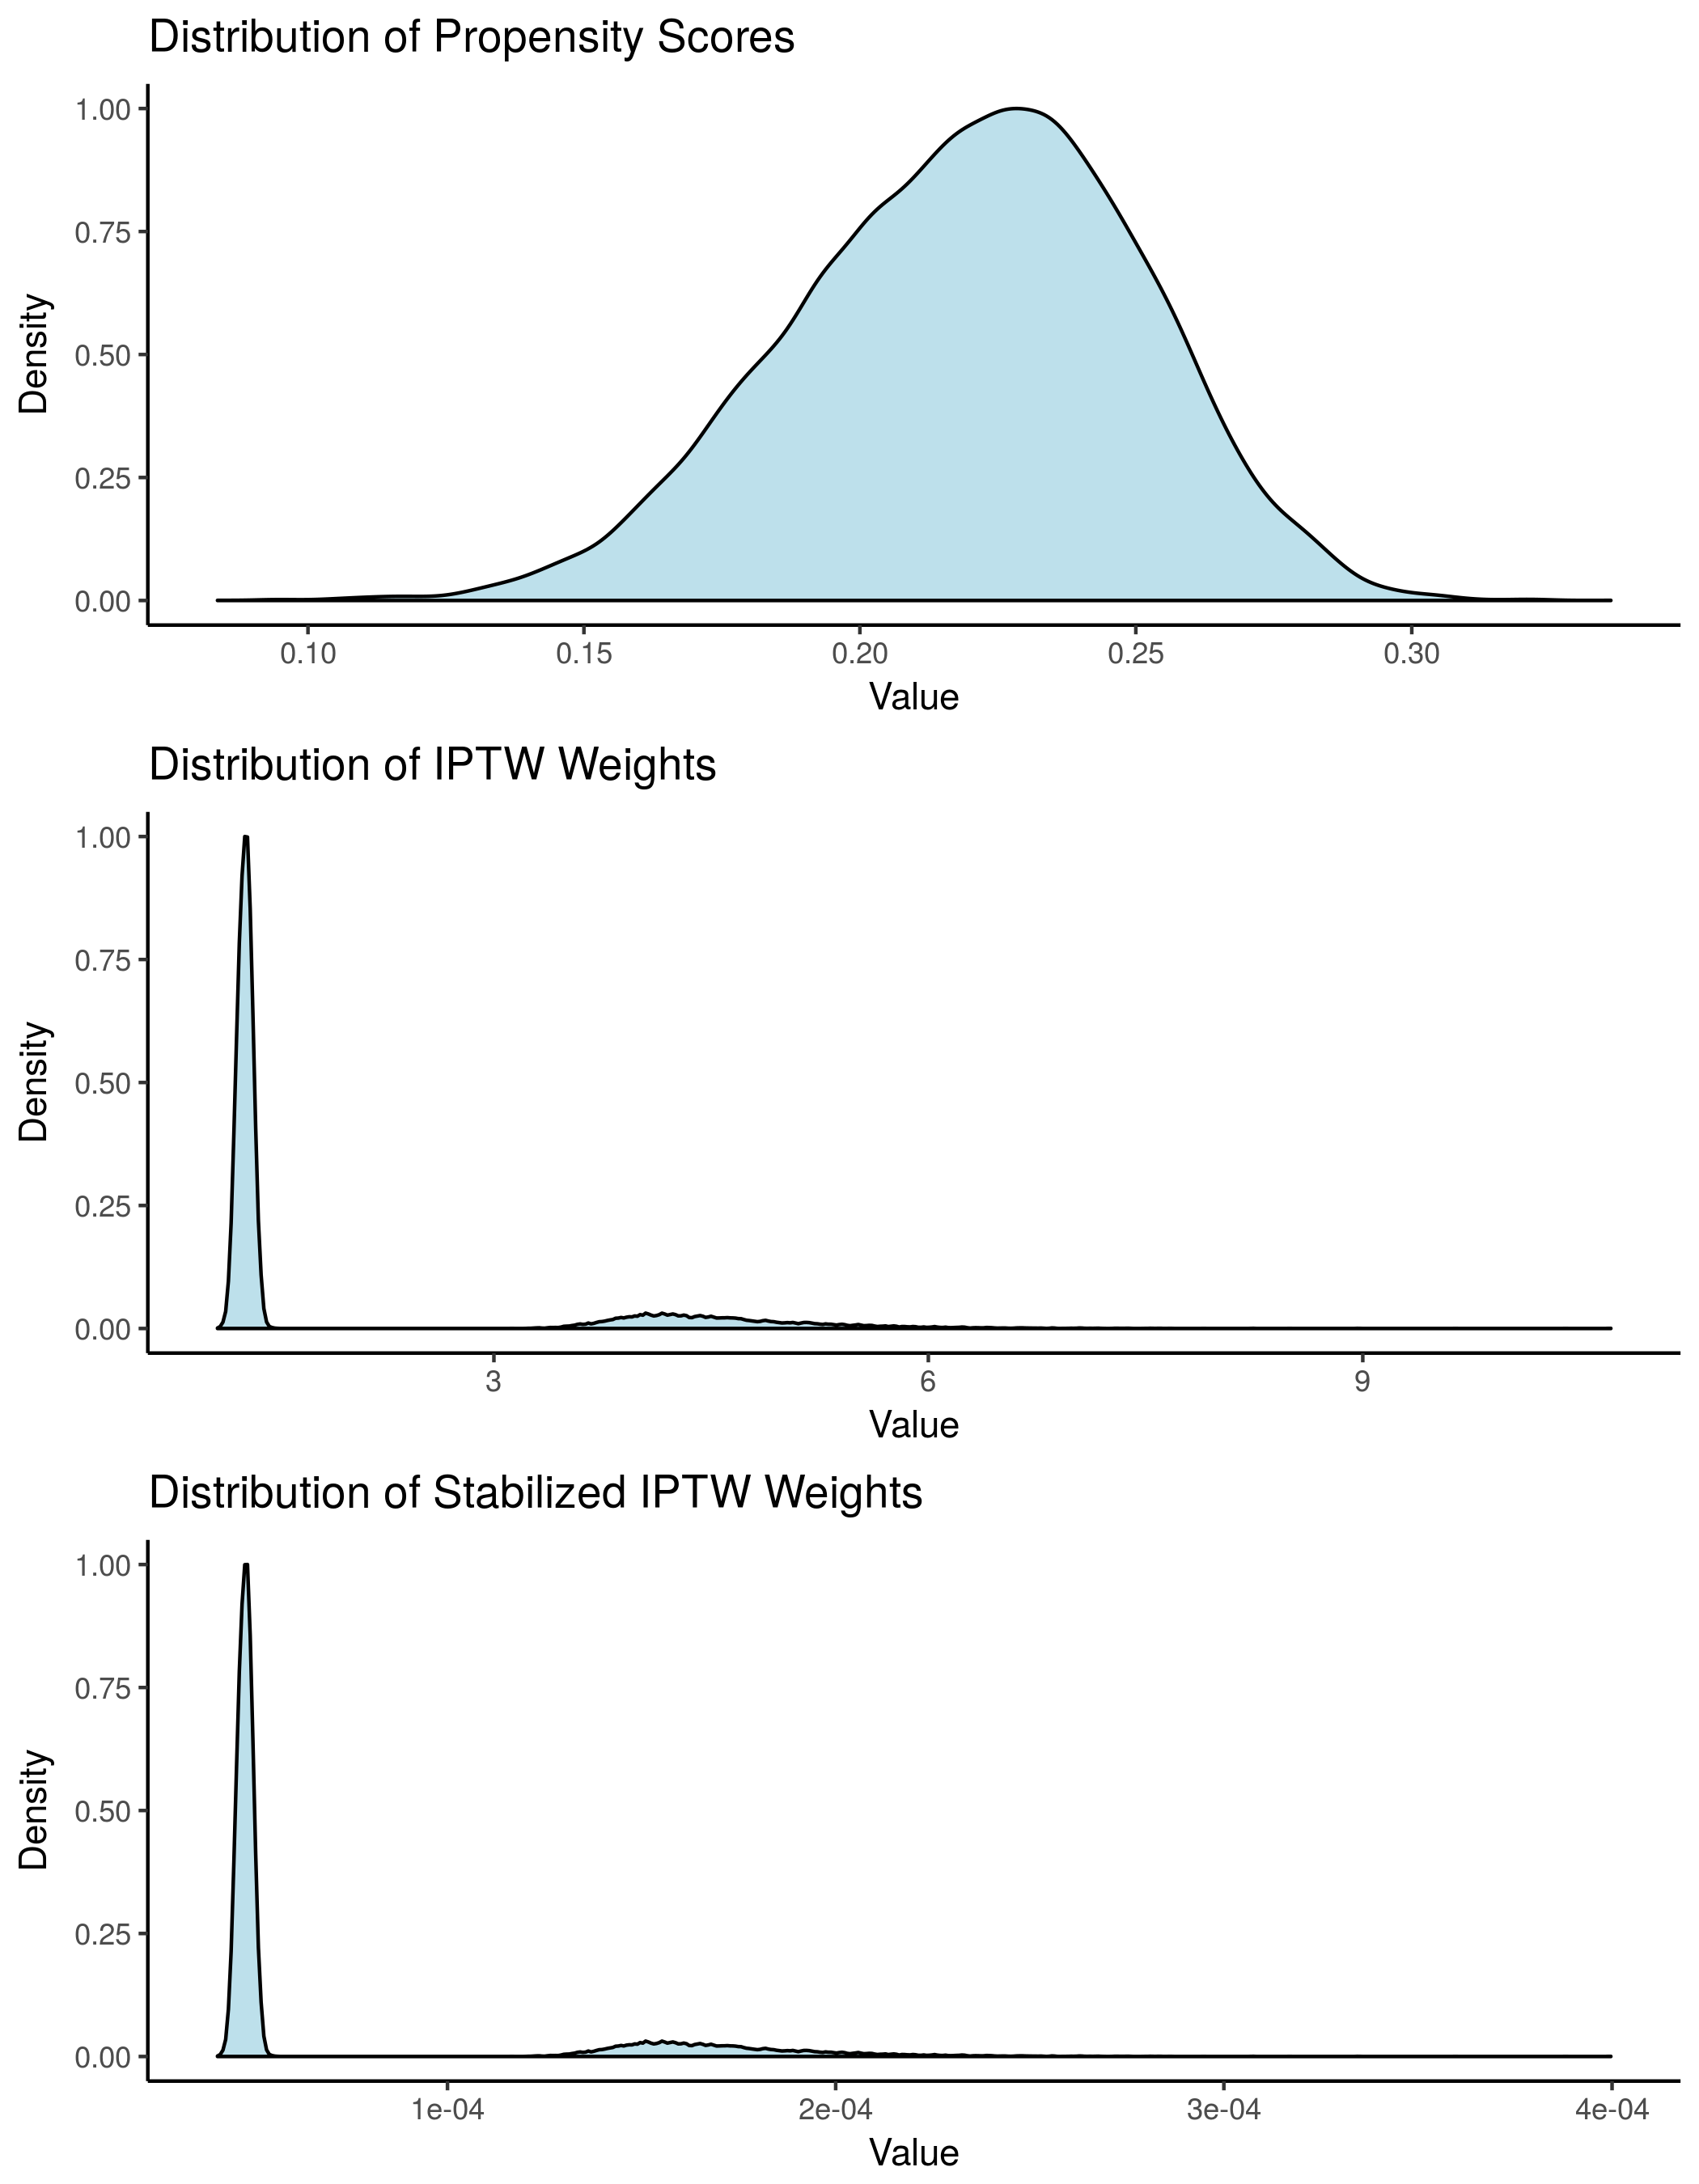
\includegraphics[scale=.35]{figures/positivity.png}
\end{minipage}\hspace{.02\columnwidth}
\begin{minipage}{0.47\columnwidth}
\begin{table}
\resizebox{\columnwidth}{!}{%
\begin{tabular}{llc}
\toprule
Propensity Scores & min  & $0.084$ \\
 & median  & $0.221$ \\  
 & mean  & $0.219$ \\
 & max  & $0.336$ \\
IPTW Weights & min  & $1.09$ \\
 & median  & $1.30$ \\
 & mean  & $2.00$ \\
 & max  & $10.7$ \\
Stabilized IPTW & min  & $4.08e-05$ \\
 & median  & $4.86e-05$ \\
 & mean  & $7.47e-05$ \\
 & max  & $4.00e-04$ \\
\bottomrule 
\end{tabular}
}
\end{table}
\end{minipage}
\end{frame}

\begin{frame}{Results}
\begin{center}
\begin{tabular}{lcccc}
\toprule
 & \multicolumn{4}{c}{Outcome} \\ \cmidrule(lr){2-5}
 & \multicolumn{2}{c}{Binary} & \multicolumn{2}{c}{Continuous} \\ \cmidrule(lr){2-3}\cmidrule(lr){4-5}
Estimand  & $\hat{\Psi}$ & SE & $\hat{\Psi}$ & \multicolumn{1}{c}{SE} \\ 
\midrule
G-Computation  & $-0.0116$ & $\phantom{-}0.00525$ & $-0.0373$ & $\phantom{-}0.0125$ \\
IPTW  & $-0.0127$ & $\phantom{-}0.00534$ & $-0.0394$ & $\phantom{-}0.0130$ \\
Stabilized IPTW  & $-0.0139$ & $\phantom{-}0.00531$ & $-0.0397$ & $\phantom{-}0.0130$ \\
TMLE (SuperLearner)  & $-0.0107$ & $\phantom{-}0.00550$ & $-0.0318$ & $\phantom{-}0.0127$
\bottomrule 
\end{tabular}
\end{center}
\end{frame}

\begin{frame}{Inference: Bootstrap Distributions Binary Response}
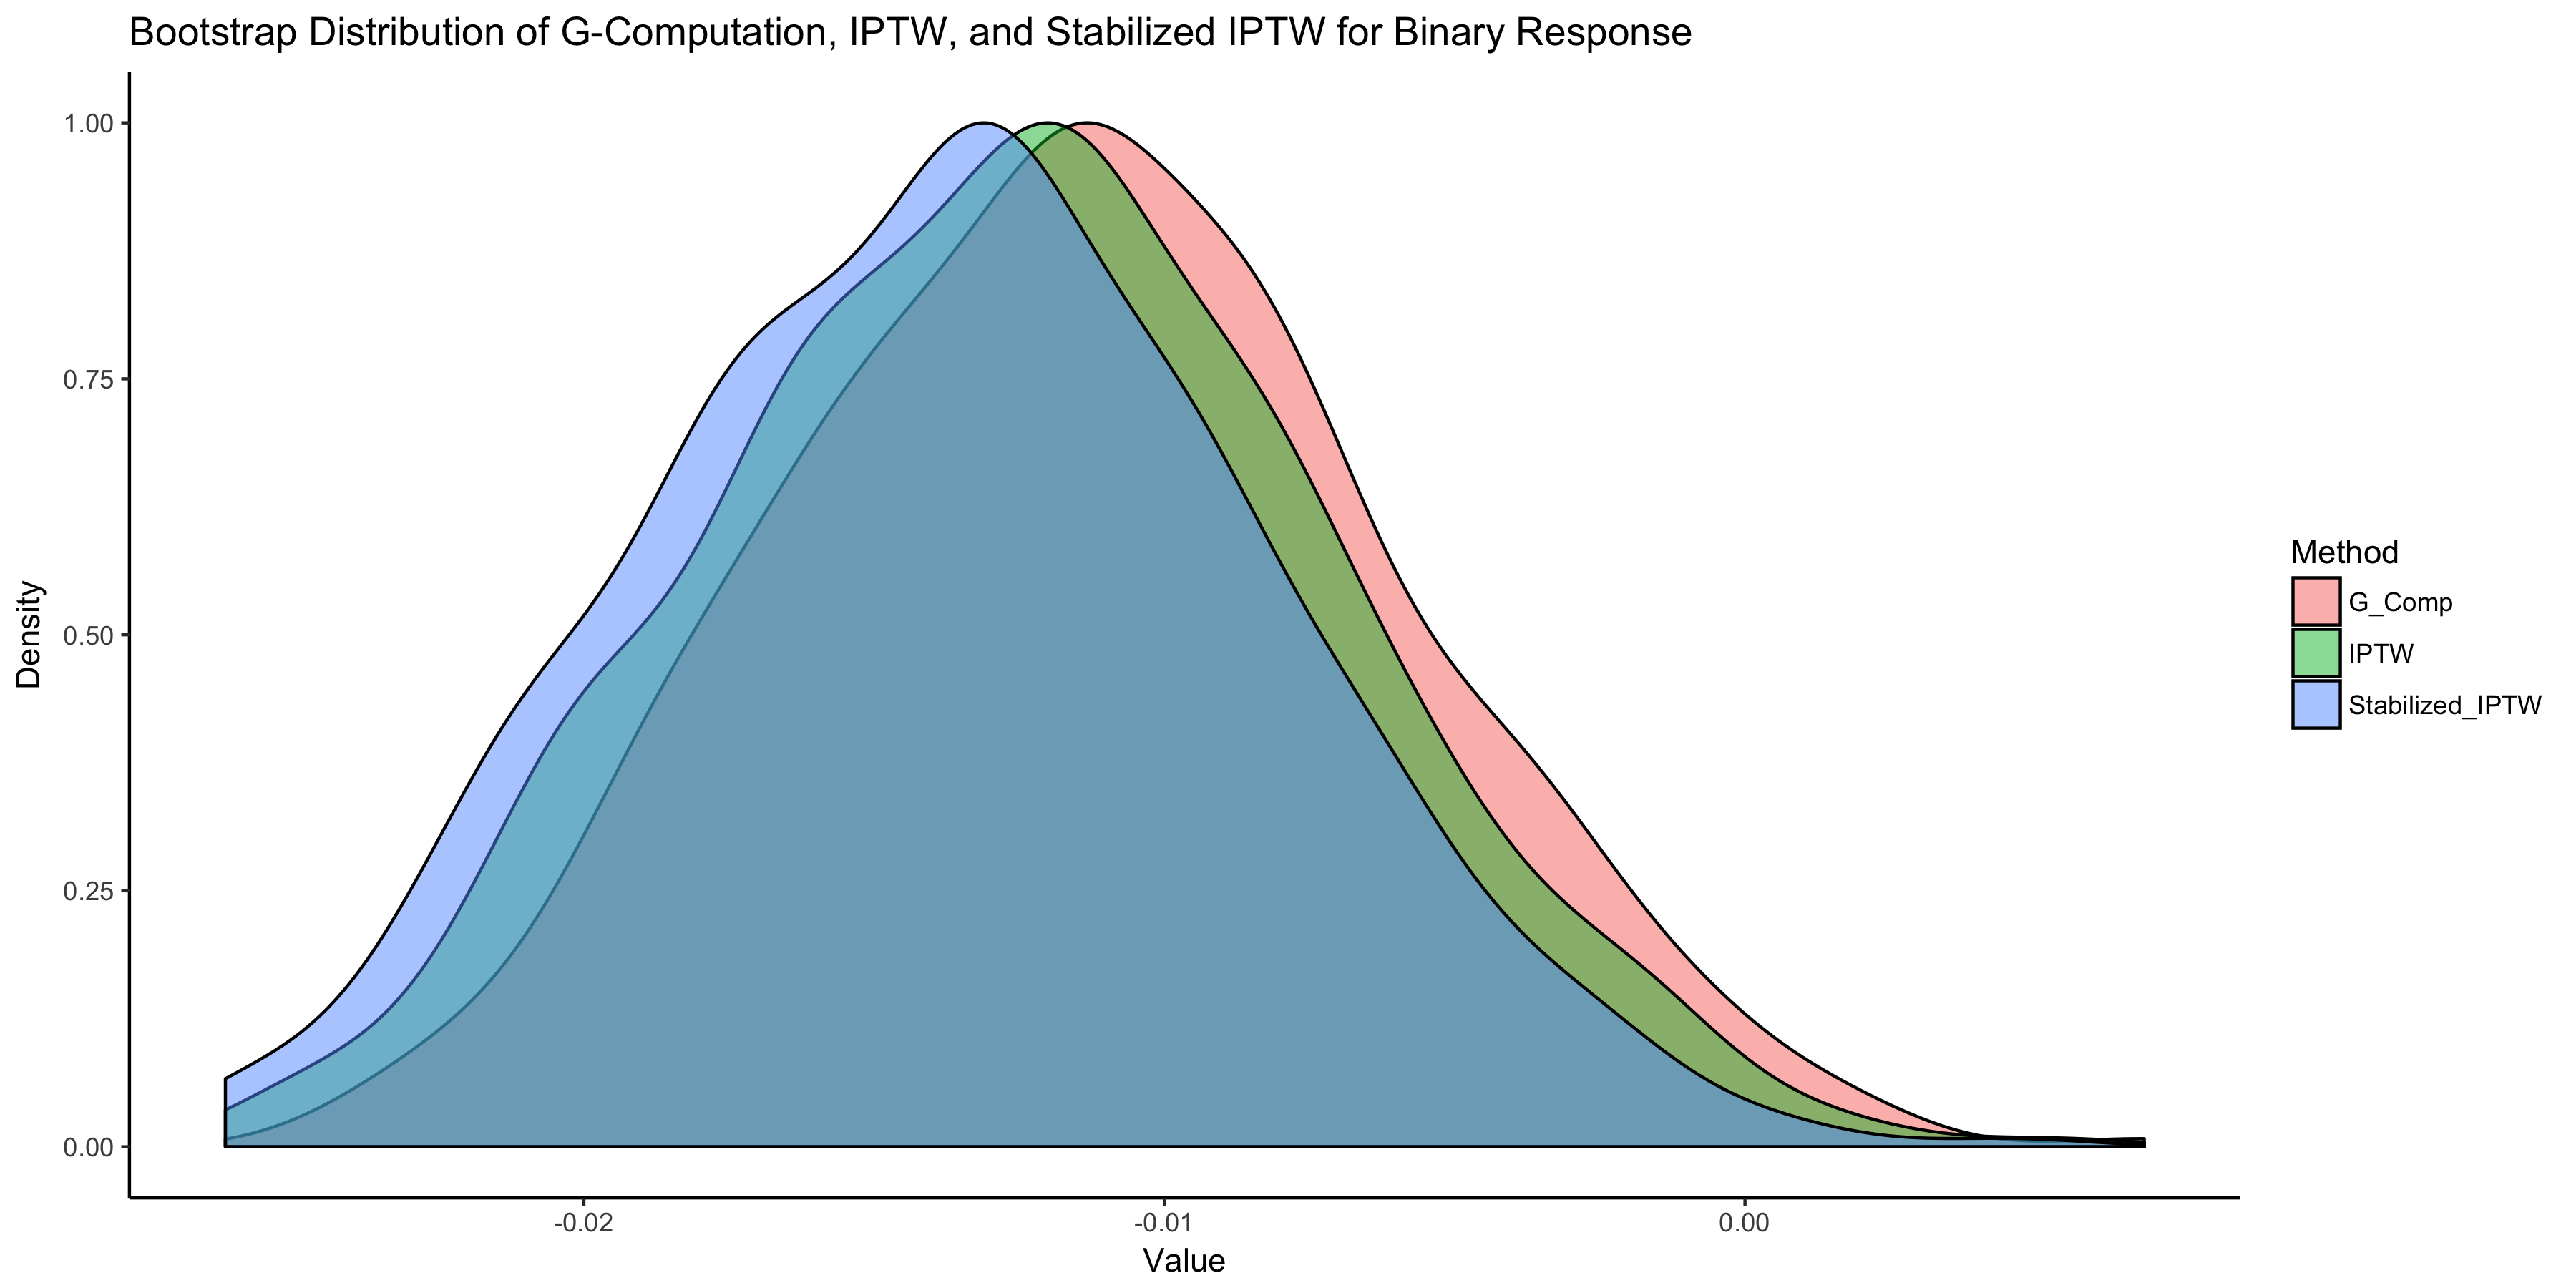
\includegraphics[scale=.095]{figures/boot_dens_binary.png}
\end{frame}

\begin{frame}{Inference: Bootstrap Distributions Continuous Response}
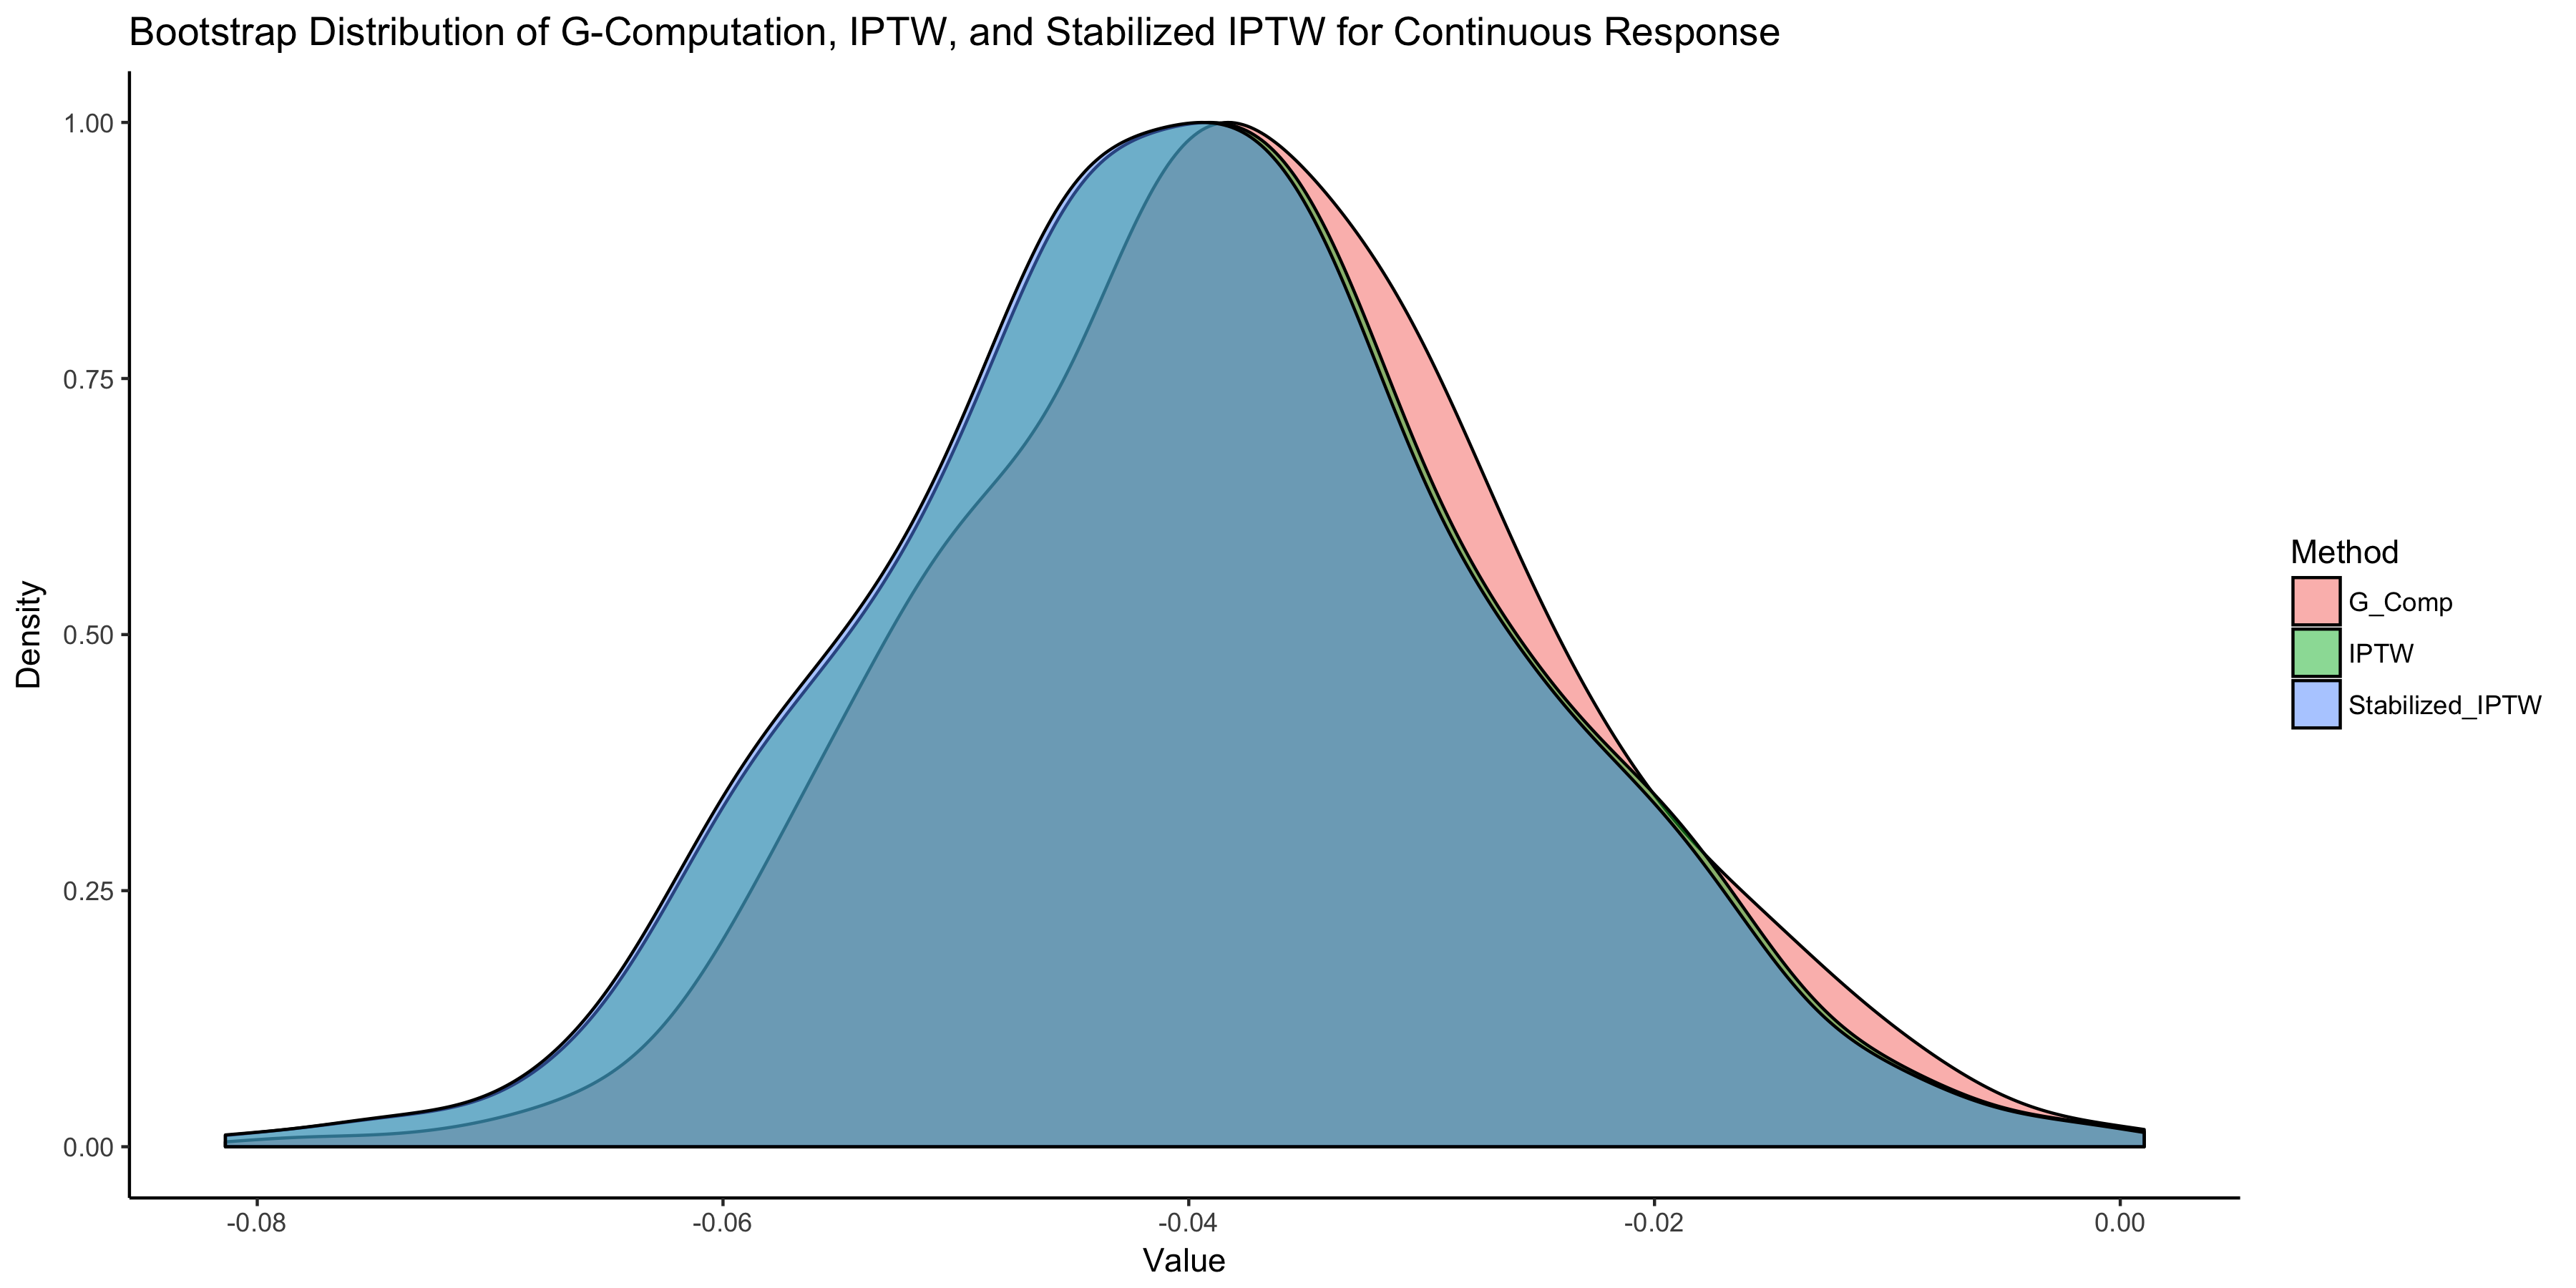
\includegraphics[scale=.095]{figures/boot_dens_continuous.png}
\end{frame}

\begin{frame}{Inference: Hypothesis Tests}
Based on our estimates and the estimated standard error, we can test whether the treatment of vaccination has a significant effect on hospitalization. Testing a two sided hypothesis, we get the following $p$-values
\begin{center}
\begin{tabular}{lcc}
\toprule
 & \multicolumn{2}{c}{Outcome} \\ \cmidrule(lr){2-3}
 & \multicolumn{1}{c}{Binary} & \multicolumn{1}{c}{Continuous} \\ \cmidrule(lr){2-2}\cmidrule(lr){3-3}
Estimand  & $p$-value & $p$-value \\ 
\midrule
G-Computation  & $0.0271$ & $\phantom{-}0.00285$ \\
IPTW  & $0.0174$ & $\phantom{-}0.00244$ \\
Stabilized IPTW  & $0.00885$ & $\phantom{-}0.00226$ \\
TMLE & $0.052$ & $\phantom{-}0.0123$ \\
\bottomrule 
\end{tabular}
\end{center}

\end{frame}

\begin{frame}{Conclusion}
In all cases, we reject the null of no effect with the treatment. Interestingly, TMLE with SuperLearner had lower significance levels, but we note that because of our small estimates and standard errors, the $p$-values were rather sensitive to small changes.

For binary response, we conclude that there is around a $1\%$ to $1.5\%$ decrease in hospitalizations for the treatment of vaccinations, whereas for continuous response, we conclude that for every 100 people who get vaccinated, there is a decrease of around 3-4 hospital visits.
\end{frame}


%%% below is an example frame
%\begin{frame}{example}
%this is text
%
%$$\text{ this is math: } \int_0^1 x dx = \frac{1}{2}$$
%
%\begin{block}{this is a block}
%This is text in a block
%$$\text{ this is math in a block: } \int_0^1 x dx = \frac{1}{2}$$
%\end{block}
%\end{frame}




\end{document}